%----------------------------------------------------------------------------
\chapter{Technologies}

In this section, I present the technologies used to build the deep learning models and to create Android and server applications.

\section{Deep learning}

I used the Python\cite{Python} programming language in deep learning-related tasks. Python is an interpreted, dynamically typed, high-level language with an object-oriented approach. Numerous libraries offer deep learning repertoire in Python, however, two libraries stand out from these: PyTorch and TensorFlow. In the following, I only describe the technologies I used during this work. My choice was driven primarily by the desire for Android interoperability, which is currently not widely supported by other tools than the selected ones.

\subsection{PyTorch}

\subsection{TensorFlow}

TensorFlow is an open-source machine learning platform developed by Google Brains. It provides rich Python and C APIs and works well with the popular Keras neural network library. TF also works well with the Colaboratory environment where GPU/TPU-based works are easy to build without local resources. In 2019, TensorFlow 2.0 has been released with Eager mode, which broke up with the former “define-and-run” scheme (where a network is statically defined and fixed, and then the user periodically feeds it with batches of training data). Eager uses a “define-by-run”approach\cite{TensorFlowEager}, where operations are immediately evaluated without building graphs.

TensorFlow uses Google’s protobuf\cite{Protobuf} format to store models. In this case, a .proto file defines a scheme, and Protocol Buffers generates the content. It is a denser format than XML or JSON, and it supports fast serialization, prevents scheme-violations, and guarantees type-safety\cite{ProtobufVsFlatbuf}. In turn, protobuf files are not as human-readable as opposed to JSON or XML.

TensorFlow Lite is a lightweight, speed, or storage optimized format aimed at deploying models on smartphones and IoT devices. Trained models can be transformed into this format with the TFLite converter. TFLite uses the Flat Buffer\cite{Flatbuf} format. It is similar to TensorFlow’s protobuf; the main difference is that Flat Buffers do not require deserializing the entire content (coupled with per-object memory allocation) before accessing an item in it. Therefore, these files consume significantly less memory than protobufs. On the other hand, Flat Buffer encoding is more complicated than in JSON/protobuf formats – for this reason, TensorFlow does not use it. It is also why TFLite models cannot be trained.

During TFLite conversion, it can be selected whether it is required to minimize model size further with a slight model accuracy trade-off or not. These are the quantization\cite{TensorFlowQuant} options used to achieve further performance gains (2-3x faster inference, 2-4x smaller networks). I used full integer quantization in which all the model maths are int8 based instead of the original float32.

The TensorBoard component provides a useful visualization tool where users see a dashboard of model performance and training/evaluation details. It can also display the current images fed to the network, the model’s answer to it, and many more. I used this tool to monitor the training/evaluation process.

\subsection{Environment}

The environment in which I worked was Google Colaboratory Pro. I was using Nvidia Tesla V100 SXM2 GPUs with 16 GB memory most of the time. At the beginning of a project, a realm is either created on or loaded from Google Drive. This is where the project saves its checkpoints and training logs. Realms are the sandboxes of notebook instances, which makes it possible to run them parallel seamlessly. In a realm, two types of projects can be - single training or hyperparameter optimization. For the latter, I used Keras Tuner.

\begin{figure}[htb]
 \centerline{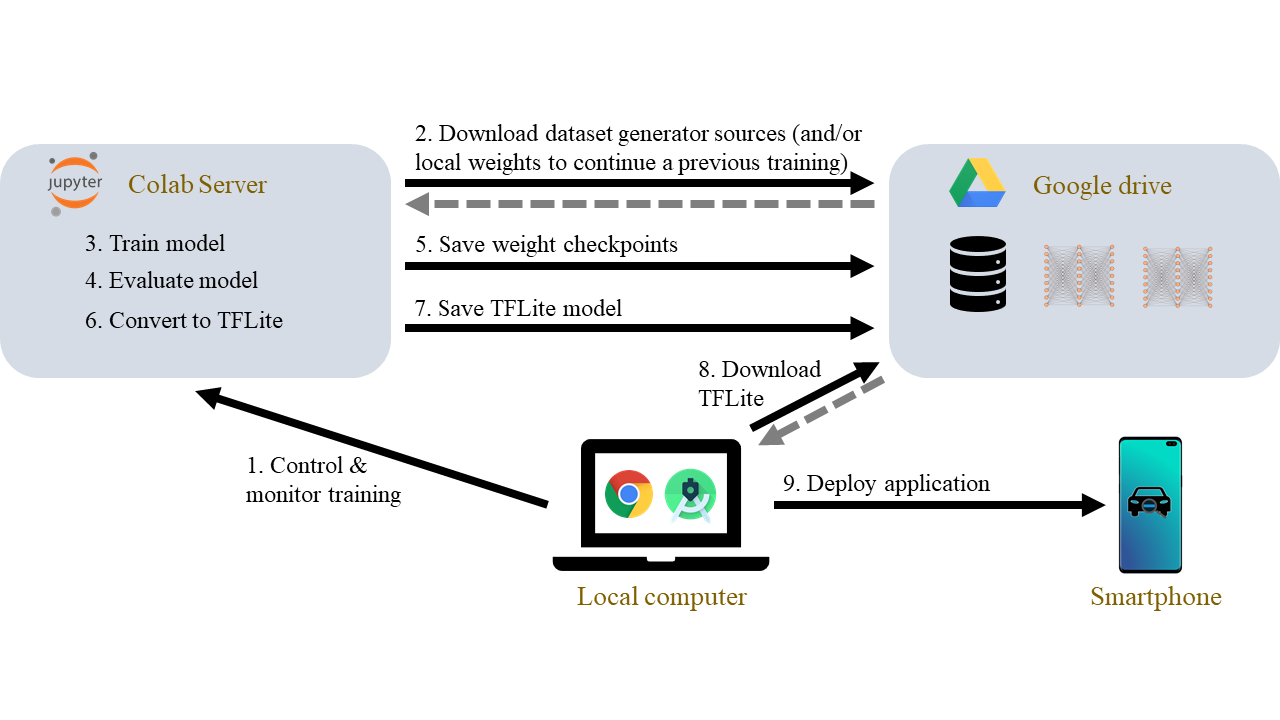
\includegraphics[width=1.0\columnwidth]{.//Figure/Technologies/Slide1.PNG}}
 \caption{High-level overview of the training environment.}
 \label{fig:simple}
\end{figure}

\pagebreak
\section{Application}

I used the Kotlin programming language\cite{Kotlin} in both the frontend and the backend. Kotlin is a statically typed, cross-platform language with type inference. In addition to the object-oriented approach, it also contains functional programming tools.

\subsection{Frontend}

Android provides an extensive application development ecosystem. I used the AndroidX namespace elements, which replaces the previous Support Library since Android 9.0. It is part of Android Jetpack, a collection of components for which the platform promises long-term support. Of these libraries, the application extensively uses the CameraX API to manage device cameras. The ViewModel component acts as a moderator between the user interface and the business logic. The app contains a relational database implemented by the Room Persistence Library, which provides an abstraction layer over SQLite to allow for more robust database access. To boost user experience, I decided to use a text-to-speech engine to read aloud alerts (useful if a user wants notifications while driving or wants to hear how to use tips). 

Material Design defines guidelines for building the interface to maximize user experience. On Android, Material elements supported by the platform can be accessed through a library. The application uses its concepts, styles, icons, fonts, and UI elements (e.g., Floating Action Button, Snackbar).

\subsection{Backend}

I used Ktor\cite{Ktor} for the backend. It is an open-source, asynchronous framework for creating microservices and web applications.JSON data handling was implemented with the Gson library. I tested the server API with Postman, and for web scraping, I used ParseHub.

